\section{Background}
\label{sec:background}

The deep learning ecosystem is embracing a rapidly growing diversity of hardware platforms including CPUs, GPUs, FPGAs, and ASICs.
In order to deploy DNNs on these platforms, high-performance tensor programs are needed for the operators used in DNNs.
The required operator set typically contains a mixture of standard operators (\textit{e.g.}, matmul, conv2d) and novel operators invented by machine learning researchers (\textit{e.g.}, capsule conv2d~\cite{hinton2018matrix}, dilated conv2d~\cite{yu2015multi}).


\begin{figure}[t]
	\centering
	\vskip -1.0em
	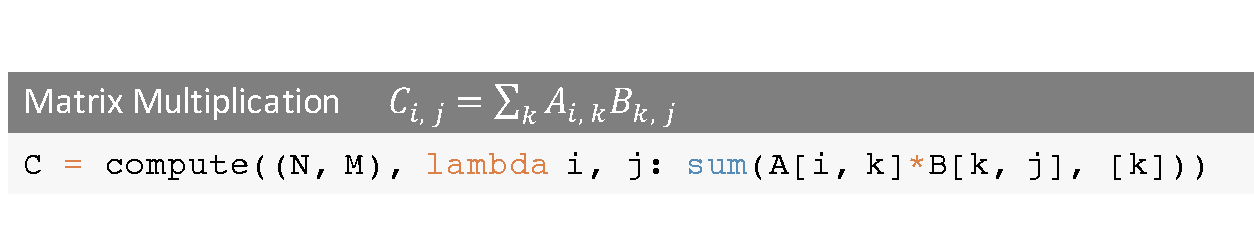
\includegraphics[width=1.01\columnwidth]{figures/compute-definition-examples.pdf}
	\precap 
	\caption{The computation definition of matrix multiplication.}
	\postcap \vskip -0.5em
	\label{fig:compute-definition-examples}
\end{figure}

To deliver portable performance of these operators on a wide range of hardware platforms in a productive way, multiple
compiler techniques have been introduced (\textit{e.g.},  TVM~\cite{chen2018tvm}, Halide~\cite{ragan2013halide}, Tensor Comprehensions~\cite{vasilache2018tensor}).
Users define the computation in a form similar to mathematical expressions using a high-level declarative language, and the compiler generates optimized tensor programs according to the definition.
\autoref{fig:compute-definition-examples} shows the computation definition of matrix multiplication in the TVM tensor expression language. Users mainly need to define the shapes of the tensors and how each element in the output tensor is computed.

However, automatically generating high-performance tensor programs from a high-level definition is extremely difficult.
Depending on the architecture of the target platform, the compiler needs to search in an extremely large and complicated space containing combinatorial choices of optimizations (\textit{e.g.}, tile structure, tile size, vectorization, parallelization).
Finding high-performance programs requires the search strategy to cover a comprehensive space and explore it efficiently.
We describe two recent and effective approaches in this section and other related work in \autoref{sec:related-work}.

\begin{figure*}[t!]
	\centering
	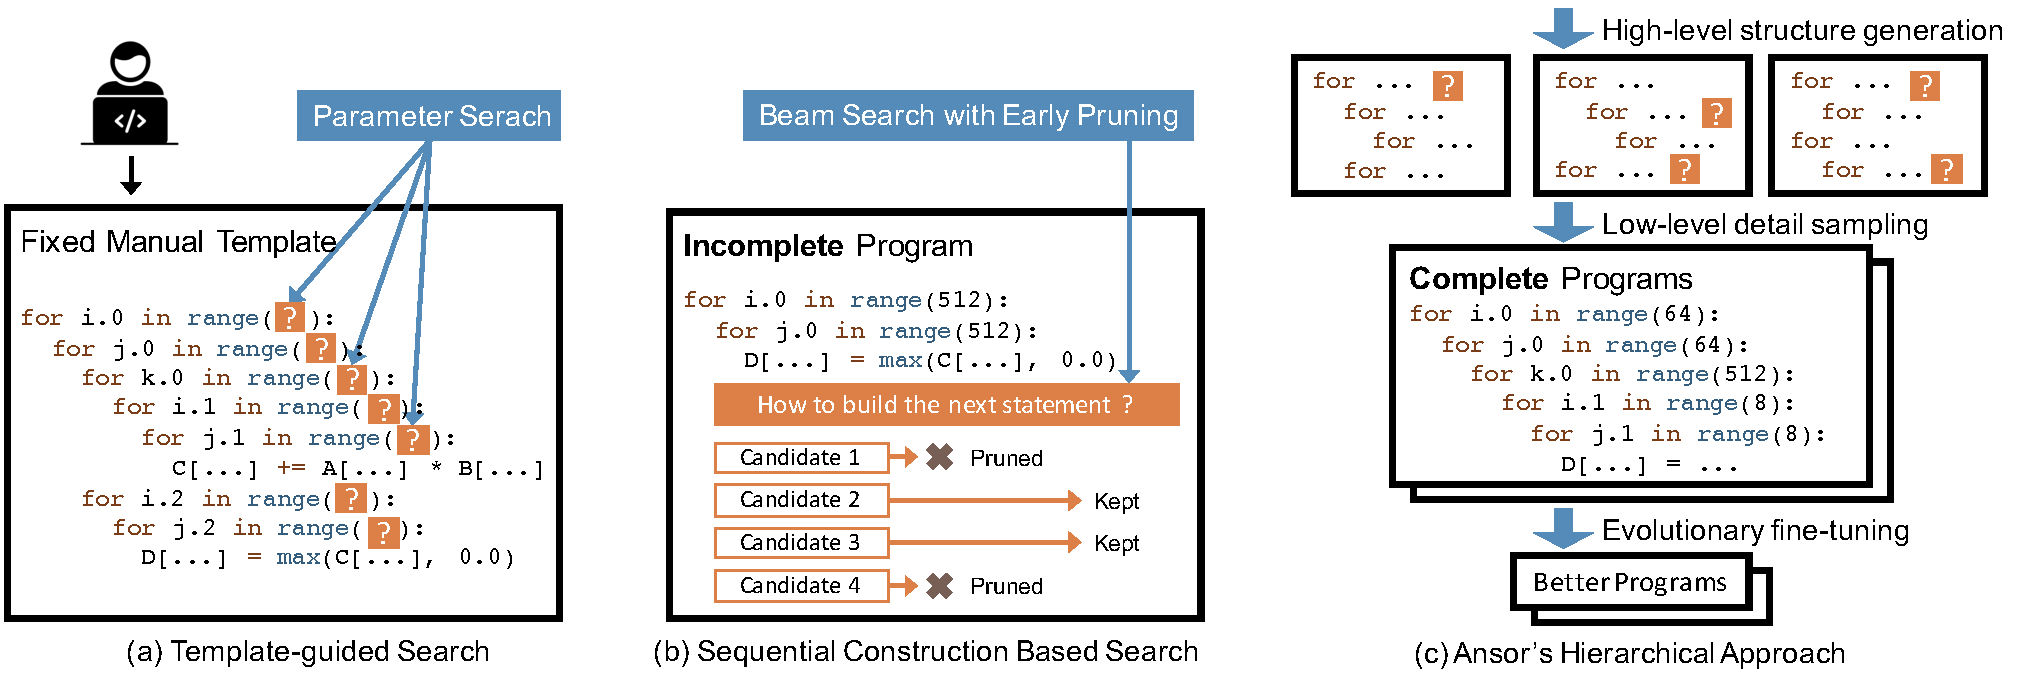
\includegraphics[width=0.95\textwidth]{figures/search-algorithm-comparison.pdf}
	\precap
	\caption{Search strategy comparison. The pseudo-code shows tensor programs with loop nests. The question marks in orange background denote low-level parameters.}
	\postcap
	\label{fig:search-algorithm-comparison}
\end{figure*}

\textbf{Template-guided search.}
In template-guided search, the search space is defined by manual templates.
As shown in \autorefsuffix{fig:search-algorithm-comparison}{a}, the compiler (\textit{e.g.}, TVM) requires the user to manually write a template for a computation definition.
The template defines the structure of the tensor programs with some tunable parameters (\textit{e.g.}, tile size and unrolling factor).
The compiler then searches for the best values of these parameters for a specific input shape configuration and a specific hardware target. 
This approach has achieved good performance on common deep learning operators.
However, developing templates requires substantial effort.
For example, the code repository of TVM already contains more than 15K lines of code for these templates. This number continues to grow as new operators and new hardware platforms emerge.
Besides, constructing a quality template requires expertise in both tensor operators and hardware. It takes non-trivial research effort ~\cite{liu2019optimizing, wang2019unified, zheng2020flextensor} to develop quality templates.
Despite the complexity of template design, manual templates only cover limited program structures because manually enumerating all optimization choices for all operators is prohibitive.
This approach typically requires defining one template for each operator.
FlexTensor \cite{zheng2020flextensor} proposes a general template to cover multiple operators, but its template is still designed for single operator granularity, which fails to include optimizations involving multiple operators (\textit{e.g.}, operator fusion).
The search space of optimizing a computational graph with multiple operators should contain different ways to compose the operators. A template-based approach fails to achieve this because it cannot break down their fixed templates and re-compose them during the search.

\textbf{Sequential construction based search.} This approach defines the search space by decomposing the program construction into a fixed sequence of decisions.  The compiler then uses an algorithm such as beam search \cite{medress1977speech} to search for good decisions (\textit{e.g.}, Halide auto-scheduler~\cite{adams2019learning}). 
In this approach, the compiler constructs a tensor program by sequentially unfolding all nodes in the computational graph. 
For each node, the compiler makes a few decisions on how to transform it into low-level tensor programs (\textit{i.e.,} deciding computation location, storage location, tile size, \textit{etc.}).
When all nodes are unfolded, a complete tensor program is constructed.
This approach uses a set of general unfolding rules for every node, so it can search automatically without requiring manual templates.
Because the number of possible choices of each decision is large, to make the sequential process feasible, this approach keeps only top-$k$ candidate programs after every decision.
The compiler estimates and compares the performance of candidate programs with a learned cost model to select the top-$k$ candidates; while other candidates are pruned. 
During the search, the candidate programs are incomplete because only part of the computational graph is unfolded or only some of the decisions are made.
\autorefsuffix{fig:search-algorithm-comparison}{b} shows this process.

However, estimating the final performance of incomplete programs is difficult in several respects:
(1) the cost model trained on complete programs cannot accurately predict the final performance of incomplete programs. The cost model can only be trained on complete programs because we need to compile programs and measure their execution time to get the labels for training.
Directly using this model to compare the final performance of incomplete programs will result in poor accuracy.
As a case study, we train our cost model (\autoref{subsec:learned-cost-model}) on 20,000 random complete programs from our search space and use the model to predict the final performance of incomplete programs. 
The incomplete programs are obtained by only applying a fraction of loop transformations of the complete programs.
We use two ranking metrics for evaluation: the accuracy of pairwise comparison and the recall@$k$ score of top-$k$ programs 
\footnote{{recall@$k$ of top-$k$ = $\frac{|G \cap P|}{k}$, where $G$ is the set of top-$k$ programs according to the ground truth and $P$ is the set of top-$k$ programs predicted by the model. \label{fn:top-k-recall-definition} }} ($k=10$).
As shown in \autoref{fig:partial-evaluation}, the two curves start from $50\%$ and $0\%$ respectively, meaning that random guess with zero information gives $50\%$ pairwise comparison accuracy and $0\%$ top-$k$ recall.
The two curves increase quickly as the programs become complete, which means the cost model performs very well for complete programs but fails to accurately predict the final performance of incomplete programs.
(2) The fixed order of sequential decisions limits the design of the search space.
For example, some optimization needs to add new nodes to the computational graph (\textit{e.g.}, adding cache nodes, using \texttt{rfactor}\cite{suriana2017parallel}). The number of decisions for different programs becomes different. It is hard to align the incomplete programs for a fair comparison.
(3) Sequential construction based search is not scalable. Enlarging the search space needs to add more sequential construction steps, which, however, leads to a worse accumulated error.


\begin{figure}[t]
	\centering
	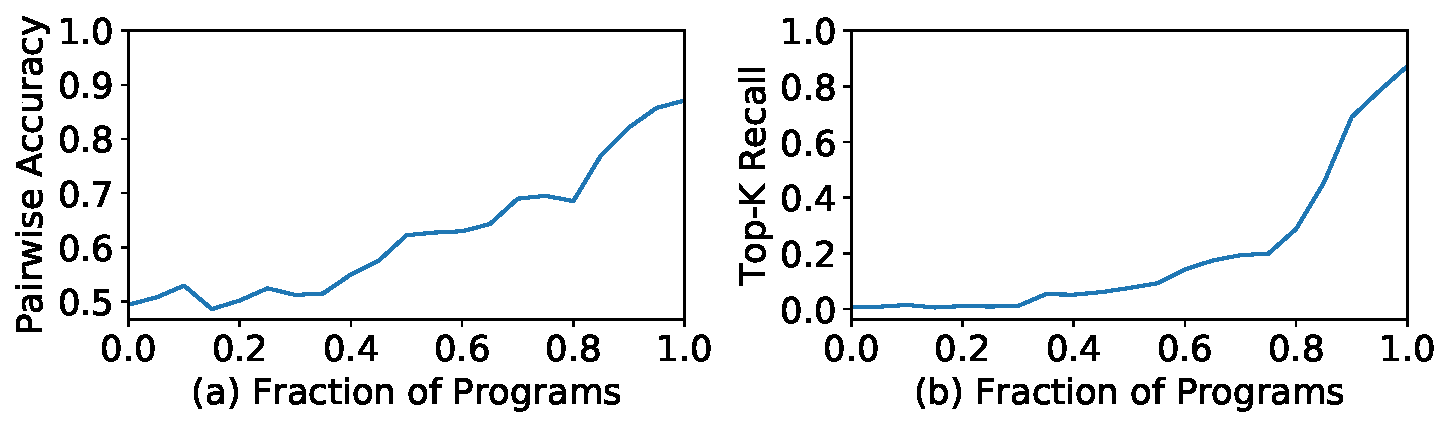
\includegraphics[width=\columnwidth]{figures/partial-estimation.pdf}
	\precap
	\caption{Pairwise comparison accuracy and top-$k$ recall curve on random partial programs. In both subfigures, higher values are better.}
	\postcap
	\label{fig:partial-evaluation}
\end{figure}


\textbf{Ansor's hierarchical approach} 
As shown in \autorefsuffix{fig:search-algorithm-comparison}{c}, \Ansor is backed by a hierarchical search space that decouples high-level structures and low-level details.
\Ansor constructs the search space for a computational graph automatically, eliminating the need to manually develop templates. \Ansor then samples complete programs from the space and performs fine-tuning on complete programs, avoiding the inaccurate estimation of incomplete programs.
\autoref{fig:search-algorithm-comparison} shows the key difference between \Ansor's approach and existing approaches.



